\section{Auswertung}
\label{sec:Auswertung}
\subsection{Acrylquader}
\subsubsection{Schallgeschwindigkeit}
Bei der Ultraschalluntersuchung des Acrylquaders wurde mittels Impuls-Echo-Verfahrens die Laufzeit der Ultraschallimpulse für verschiedene Fehlstellen im Acrylquader gemessen. Dazu wurden die Positionen der Fehlstellen mit einer Schieblehre ausgemessen. Da der Acrylquader 9 Fehlstellen hat und von 2 Seiten gemessen wurde ergeben sich 18 Datenpaare. Die Aufnahmen des A-Scans sind im Anhang zu finden. In \autoref{tab:mess} sind die Ergebnisse mit der gemessenen Position der Fehlstelle und der Laufzeit des Ultraschallimpulses aufgelistet.
\begin{table}
  \centering
  \caption{Messergebnisse zum Acrylquader}
\label{tab:mess}
  \sisetup{table-format=2.1}
  \begin{tabular}{c c }
  \toprule
  Position der Fehlstelle[$mm$] & Laufzeit Ultraschallimpuls [$\mu s$]\\
  \midrule
  7 & 5,9 \\
  15,2 & 11,8 \\
  23,2 & 17,5 \\
  30,9 & 23,35 \\
  39,2 & 29,2 \\
  46,4 & 34,5 \\
  54,4 & 40 \\
  61,45 & 45,4 \\
  55,65 & 41,2 \\
  70,65 & 46,8 \\
  62,6 & 46,5 \\
  54,55 & 40,7 \\
  46,55 & 34,9 \\
  38,6 & 29,1 \\
  30,25 & 22,9 \\
  21,7 & 16,8 \\
  13,2 & 10,5 \\
  15,45 & 11,9 \\
  \bottomrule
  \end{tabular}
\end{table} 
\newpage
Aus diesen Daten lässt sich nach ... mit einer linearen Ausgleichsrechnung die Schallgeschwindigkeit in dem Acrylquader berechnen. Dies wird in \autoref{fig:quader} dargestellt.
\begin{figure}[H]
  \centering
  \includegraphics[width=\textwidth]{build/plot.pdf}
  \caption{Diagramm: Position der Fehlstellen(s)-Laufzeit des Ultraschall Impulses(t), mit Ausgleichsgerade}
  \label{fig:quader}
\end{figure}

Die lineare Ausgleichsrechnung mit Python ergibt für die Parameter der Geraden:\newline
a=(1.41789 $\pm$ 0.03051) $\frac{mm}{\mu s}$(Steigung)\newline
b=-(1.92975 $\pm$ 0.95282) $mm$(y-Achsenabschnitt)\newline
Diese Steigung entspricht also einer Schallgeschwindigkeit von:
\begin{equation*}
  c=2*a= (2835.78 \pm 61.02) \frac{m}{s}
\end{equation*} 
\subsubsection{Dämpfung}
Zur Bestimmung des materialspezifischen Schwächungskoeffizienten von Acryl wurde die Schwächung der Amplitude der Pulse zwischen einer Fehlstelle und dem Ende des Acrylquaders untersucht. In wurden dazu jeweils beide Amplituden und die ausgemessene Distanz der beiden Stellen aufgelistet.
\begin{table}
  \centering
  \caption{Messdaten zur Dämpfung}
\label{tab:messd}
  \sisetup{table-format=2.1}
  \begin{tabular}{c c c}
  \toprule
  Amplitude1 [$V$] & Amplitude2 [$V$] & Distanz[$mm$]\\
  \midrule
1.196 0.445 48.65\\
1.168 0.385 65.3\\
0.9 0.569 57.3\\
0.841 0.403 49.6\\
0.975 0.477 41.3\\
0.927 0.354 34.1\\
0.852 0.253 26.1\\
0.645 0.244 19.1\\
1.229 0.219 65.05\\
0.435 0.258 17.9\\
0.683 0.205 25.95\\
0.984 0.194 33.95\\
1.098 0.226 41.9\\
0.798 0.274 50.25\\
1.229 0.219 65.05\\
0.994 0.145 67.3\\
  \bottomrule
  \end{tabular}
\end{table}

\subsection{Augenmodell}
In \autoref{fig:auge} sind die Ergebnisse der Untersuchung des Augenmodells mit einem A-Scan mit Impuls-Echo-Verfahren zu sehen.
\begin{figure}[H]
  \centering
  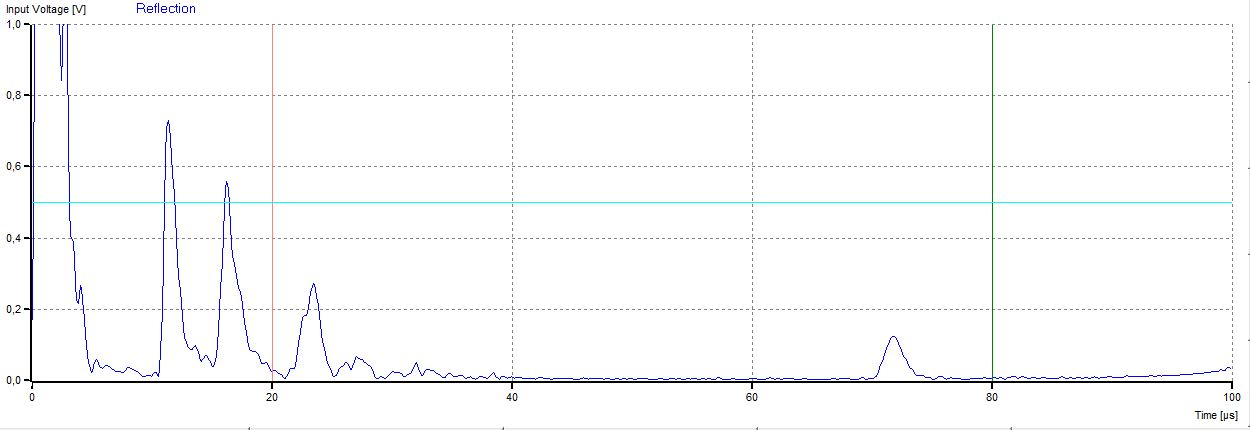
\includegraphics[width=\textwidth]{messungen/auge/auge.jpg}
  \caption{Spannungs-Zeit Diagramm zum A-Scan des Augenmodells}
  \label{fig:auge}
\end{figure}

Die ersten beiden in \autoref{fig:auge} zu sehenden Peaks werden als der Ein- und Austritt des Ultraschalls in die bzw. aus der Linse interpretiert. Der dritte Peak entspricht dem Echo des Ultraschalls von der Rückwand der Retina. Mit den bekannten Schallgeschwindigkeiten für die Linse ($c_{L} = 2500 m/s$) und die Glaskörperflüssigkeit ($c_{GK} = 1410 m/s$) sowie den Daten des A-Scans lassen sich die Abmessungen des Augenmodells berechnen. Aus den Messdaten konnten die Zeiten der 3 Peaks ermittelt werden:\newline
1.Peak: $11,4 \mu s$ \newline 2.Peak: $16,3 \mu s$ \newline 3.Peak: $23,2 \mu s$ \newline
Mit ergeben sich für die Maße des Augenmodells:
\begin{table}
  \centering
  \caption{Abmessungen des Augenmodells}
\label{tab:mess2}
  \sisetup{table-format=2.1}
  \begin{tabular}{c c c}
  \toprule
  Strecke & Zeit $[\mu s]$ & Weg[$mm$]\\
  \midrule
  Hornhaut-Linse & 11,4 & 8,037 \\
  Innerhalb der Linse & 4,9 & 6,125\\
  Linse-Retina & 6,9 & 4.865\\
  \bottomrule
  \end{tabular}
  \end{table}